
\begin{figure}
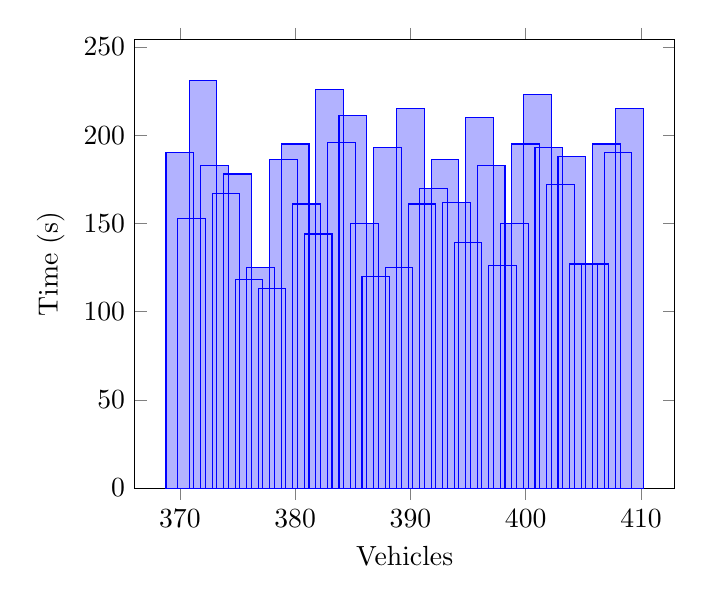
\begin{tikzpicture}
\begin{axis}[
legend style={anchor=west},
xlabel=Vehicles,
ylabel=Time (s),
ymin=0,
ybar,
]
\addplot coordinates {
(409, 215)
(407, 195)
(406, 127)
(405, 127)
(403, 172)
(402, 193)
(401, 223)
(400, 195)
(379, 186)
(378, 113)
(370, 190)
(377, 125)
(376, 118)
(393, 186)
(392, 170)
(397, 183)
(396, 210)
(395, 139)
(394, 162)
(398, 126)
(391, 161)
(380, 195)
(381, 161)
(382, 144)
(383, 226)
(384, 196)
(385, 211)
(386, 150)
(387, 120)
(388, 193)
(389, 125)
(404, 188)
(408, 190)
(371, 153)
(373, 183)
(375, 178)
(374, 167)
(390, 215)
(372, 231)
(399, 150)
};

\end{axis}
\end{tikzpicture}
\label{tik:time:0:96}
\caption{0 percent diving with GSC on route $96$}
\end{figure}
